%:
% !TEX TS-program = pdflatex
% !TEX encoding = UTF-8 Unicode

% This is a simple template for a LaTeX document using the "article" class.
% See "book", "report", "letter" for other types of document.

%\documentclass{scrartcl}
\documentclass[11pt]{article} % use larger type; default would be 10pt
%\setkomafont{disposition}{\normalfont\bfseries}	

\usepackage[utf8]{inputenc} % set input encoding (not needed with XeLaTeX)

%%% PAGE DIMENSIONS
\usepackage{geometry} % to change the page dimensions
\usepackage{amsmath}
\geometry{a4paper} % or letterpaper (US) or a5paper or....
% \geometry{margin=2in} % for example, change the margins to 2 inches all round
% \geometry{landscape} % set up the page for landscape
%   read geometry.pdf for detailed page layout information

\usepackage{booktabs}% http://ctan.org/pkg/booktabs

\usepackage{graphicx} % support the \includegraphics command and options
\usepackage{natbib} % support the \includegraphics command and options
\usepackage{xcolor,colortbl}

\usepackage{multicol}

% \usepackage[parfill]{parskip} % Activate to begin paragraphs with an empty line rather than an indent

%%% PACKAGES
\usepackage{booktabs} % for much better looking tables
\usepackage{array} % for better arrays (eg matrices) in maths
\usepackage{paralist} % very flexible & customisable lists (eg. enumerate/itemize, etc.)
\usepackage{verbatim} % adds environment for commenting out blocks of text & for better verbatim
\usepackage{subfigure} % make it possible to include more than one captioned figure/table in a single float
% These packages are all incorporated in the memoir class to one degree or another...

%%% HEADERS & FOOTERS
\usepackage{fancyhdr} % This should be set AFTER setting up the page geometry
\pagestyle{fancy} % options: empty , plain , fancy
\renewcommand{\headrulewidth}{0pt} % customise the layout...
\lhead{}\chead{}\rhead{}
\lfoot{}\cfoot{\thepage}\rfoot{}

%%% SECTION TITLE APPEARANCE
\usepackage{sectsty}
\allsectionsfont{\sffamily\mdseries\upshape} % (See the fntguide.pdf for font help)
% (This matches ConTeXt defaults)

%%% ToC (table of contents) APPEARANCE
\usepackage[nottoc,notlof,notlot]{tocbibind} % Put the bibliography in the ToC
\usepackage[titles,subfigure]{tocloft} % Alter the style of the Table of Contents
\renewcommand{\cftsecfont}{\rmfamily\mdseries\upshape}
\renewcommand{\cftsecpagefont}{\rmfamily\mdseries\upshape} % No bold!

\newcommand{\sw}{\textit{software}\xspace}
\newcommand{\sws}{\textit{softwares}\xspace}
\newcommand{\iso}{ISO 29110\xspace}

\usepackage{titling}
\usepackage[brazil]{babel}
\usepackage{xspace}

\usepackage{framed}

\usepackage{setspace}
\onehalfspacing

\usepackage{url}

%\DeclareUnicodeCharacter{00A0}{ }

%%% END Article customizations

%%% The "real" document content comes below...

\begin{document}

%\inputencoding{latin1}\input{titulo}
% !TEX root = Monografia Mestrado.tex

\chapter{Introdução}

\section{Engenharia de \sw}

De acordo com \cite{pressman}, a engenharia de \sw é uma tecnologia em camadas e qualquer abordagem de engenharia deve se apoiar em um compromisso organizacional com a \textbf{qualidade} e com um processo contínuo de aperfeiçoamento, como ilustrado na Figura \ref{fig:sw.camadas}. Algumas ferramentas da administração e filosofias, tais como Gestão da Qualidade Total\footnotemark \footnotetext{\textit{Total Quality Management} (TQM) consiste numa estratégia de administração orientada a criar consciência da qualidade em todos os processos organizacionais.}, Seis Sigma\footnotemark \footnotetext{\textit{Six Sigma} é um conjunto de práticas originalmente desenvolvidas pela Motorola para melhorar sistematicamente os processos ao eliminar defeitos.} e Manufatura Enxuta\footnotemark, podem instituir a cultura de qualidade necessária para esta indústria.

\footnotetext{\textit{Lean Manufacturing} ou Sistema Toyota de Produção é uma filosofia de gestão focada na redução de desperdícios.}

\begin{figure}[!h]
\centering

\includegraphics[scale=1]{figuras/eng_sw_camadas.png}
\caption{Camadas da engenharia de \sw \citep[p.17]{pressman}}
%http://www.devmedia.com.br/principios-da-engenharia-de-software/29630
\label{fig:sw.camadas}
\end{figure}

As próxima camada, \textbf{processo}, define regras e padrões que permitem o controle e gerência dos projetos de desenvolvimento, além de estabelecer o contexto no qual as próximas camadas irão atuar. Os \textbf{métodos} oferecem técnicas de construção dos \sws (como fazer) e as \textbf{ferramentas} fornecem apoio para as primeiras camadas e podem ser automatizadas ou semi-automatizadas, integradas ou não, gratuitas ou pagas, etc.

Alguns problemas antigos da engenharia de \sw, que teve seu início na década de 50, ainda convivem com as empresas desenvolvedores nos dias atuais: precariedade  nas  previsões  e  planejamentos, baixa qualidade de processos e produtos, requisitos  mal  definidos e o alto custo para manutenção. Tais problemas podem ser atribuídos à gestão ineficiente ou inadequada dos projetos e consomem recursos importantes (humanos e financeiros, principalmente) por conta do retrabalho.

\section{Representatitividade e dificuldades das VSEs}

A indústria de \sw representa 8\% do PIB e 6\% dos postos de trabalho na Europa e pequenas e médias empresas de desenvolvimento respondem por 90\% dos negócios formais que geram entre 40\% e 50\% do total de empregos \citep{reicis}. Empresas com 10 ou menos funcionários representam 85\% do total na Europa e 50\% em Montreal, Canadá, considerando somente empresas de TI e 93\% na Europa e 50\% nos Estados Unidos, considerando qualquer tipo de empresa \citep{ieee_comp}. 

O Brasil, que em 2011 passou a ocupar a 10\textsuperscript{a} posição no \textit{ranking} mundial de \sw e serviços com um faturamento de cerca de US\$ 21 bilhões de dólares, possui 97,3\% das quase 70 mil empresas do setor classificadas como Micro e Pequeno Empresas (MPE) com até 19 pessoas \citep{guia.sebrae}.

Apesar de representativas, estudos apontam que estas pequenas e médias empresas de \sw não são atendidas por normas e padrões que se encaixem em suas realidades. Padrões internacionais, como ISO e IEEE, apresentam diversas barreiras econômicas e operacionais que tornam virtualmente impossível a sua implementação por uma VSE.

De acordo com \cite{fayad}, existem quatro questões que não são tratadas de forma adequada pela literatura na área de engenharia de \sw:

\begin{itemize}

\item[\textbf{Tamanho da empresa}]: indústria, governo, associações e outras instituições podem definir números diferentes para designar que uma empresa é pequena, podendo variar de 10 a 500 funcionários ou mais. Além disso, empresas que não possuem foco somente no desenvolvimento de \sw podem possuir um contingente muito grande de funcionários, porém somente um pequeno percentual deste total dedicado às atividades de \sw.

\item[\textbf{Modo de desenvolvimento}]: o modelo de contrato sugerido pela literatura, onde o cliente do \sw é identificado, mesmo que seja um departamento dentro de uma empresa, nem sempre funciona para pequenas empresas. Estas, geralmente, não se utilizam de contratos formais, não conseguem identificar ou isolar bem o cliente ou simplesmente os profissionais de TI não ``perdem tempo'' com isso porque precisam manter o foco nas especificações do produto.

\item[\textbf{Velocidade de desenvolvimento}]: competitividade acirrada e demanda de entregas rápidas pelo mercado frutificaram em novas estratégias rápidas de desenvolvimento.
 
\item[\textbf{Tamanho de desenvolvimento}]: hoje o número de linhas de código dos \sws considerados pequenos supera o número de linhas dos \sws considerados grandes no passado. Isso incorre no fato que pequenas empresas começam a necessitar de metodologias de \sw desenvolvidas para projetos de larga escala que, infelizmente, não se apadtam bem aos projetos de pequena escala.
 
\end{itemize}

Como tentativa de contornar as principais barreiras e tratar de melhor forma as questões citadas acima, algumas propostas de melhoria dos processos de desenvolvimento de \sw foram adotados ao redor do mundo, sendos os principais:

\begin{itemize}

\item[\textbf{SPIRE\footnotemark e TOPS\footnotemark}] promovidos pela União Europeia através do \textit{European Software and System Initiative} (ESSI);

\item[\textbf{MoProSoft}] adotado pelo México para a indústria de \sw, baseado na ISO 12207, CMM e ISO 9001;

\item[\textbf{EvalProSoft}] também adotado pelo México, baseado na ISO 15504;

\item[\textbf{MPS-BR}] no Brasil tem como método de avaliação o MA-MPS, baseado na ISO 15504;

\item[\textbf{COMPETISOFT}] estabelecido na Iberoamérica, que tem seu modelo de referência baseado na ISO 12207, CMM, ISO 9001, MANTEMA  e métrica V3, seu método de avaliação sugerido baseado na ISO 15504 e seu modelo de gestão de melhora influenciado pelo IDEAL e SCRUM;

\item[\textbf{IPRC}] é o Consórcio Internacional de Investigação de Processos criado pelo SEI com o objetivo de melhorar processos para os chamados \textit{Small Settings} (IPSS), referentes aos projetos com menos de 20 pessoas, organizações com menos de 50 pessoas e/ou empresas com menos de 100 pessoas;

\item[\textbf{I.T.Mark}] foi desenvolvido e aplicado na Europa, Ásia e Iberoamérica pelo ESI e se baseia no CMMI e ISO 17799:2005.

\end{itemize}

\footnotetext[1]{\url{http://www.cse.dcu.ie/spire/}} 

\footnotetext{\url{http://cordis.europa.eu/esprit/src/27977.htm}} 

\section{História da \iso}

Em 2004, durante a reunião plenária do SC7\footnotemark{} na Austrália, delegados de cinco nações chegaram a um consenso a respeito da necessidade da criação de padrões internacionais que atendessem ao tamanho e particularidades das VSEs. Os padrões deveriam incluir perfis e guias e o grupo chegou a um acordo sobre os seguintes objetivos gerais:

\footnotetext{ISO/IEC JTC 1/SC 7 \textit{Software and systems engineering} -  \url{http://www.iso.org/iso/iso_technical_committee?commid=45086}}

\begin{itemize}

\item Fazer com que os padrões atuais de engenharia de \sw fossem mais acessíveis às VSEs;

\item Fornecer documentações que requeiram o mínimo de esforço em adaptações;

\item Fornecer documentações harmonizadas integrando padrões já disponíveis como padrões de processos, produtos de trabalho e entregáveis, ferramentas de avaliações, qualidade e modelagem;

\item Levar em consideração, se desejável, as noções de níveis de capacidade e maturidade apresentados na ISO/IEC 15504 e no CMMI.

\end{itemize}

Em 2005, na reunião plenária do SC7 na Finlândia, a Tailândia propôs a criação de um grupo de trabalhos para atingir estes objetivos, que foi aprovada por doze países e estabeleceu o \textit{Working Group} 24 (WG24) com os seguintes países membros: Bélgica, Canadá, República Tcheca, Irlanda, Itália, Japão, Coréia, Luxemburgo, África do Sul, Tailândia, Reino Unido e os Estados Unidos.

Uma pesquisa foi conduzida pelo WG24 para refinar os requisitos das VSEs e estas foram questionadas sobre a sua utilização dos padrões ISO/SC7 e também sobre problemas e possíveis soluções que poderiam ajudar na aplicação de padrões e torná-las mais competitivas. O Brasil foi o país com o segundo maior número de respostas, totalizando 68, perdendo somente para a Colômbia, com 88. O objetivo desta pesquisa foi validar algumas hipóteses, incluindo:

\begin{itemize}

\item O contexto das VSEs requer perfis de ciclo de vida leves e muito bem focados;

\item Contextos de negócio particulares requerem perfis particulares;

\item Existem diferenças significantes em termos de recursos e infraestrutura disponíveis entre uma VSE que emprega de 1 a 10 pessoas e um departamento de TI do mesmo tamanho em uma empresa grande;

\item As VSEs são limitadas em tempo e recursos, o que leva a uma falta de entendimento sobre como os uso dos padrões podem beneficiá-las;

\item Os benefícios para VSEs podem incluir reconhecimento através de avaliacões ou auditorias realizadas por um órgão acreditado.

\end{itemize}

A pesquisa incluiu propositalmente questionamentos sobre o porquê da pouca adoção de padrões e descobriu-se que eram três os principais motivos: 

\begin{itemize}

\item Falta de recursos - 28\%;

\item Não eram necessários - 24\%;

\item A natureza em si dos padrões - 15\% (consideravam os padrões difíceis e burocráticos e não forneciam acompanhamento adequado para uso em pequenos ambientes empresariais).

\end{itemize}

Apesar disso, uma maioria de três quartos achavam importante serem avaliadas ou certificadas em um padrão, sendo a certificação ISO mencionada por 40\% dos entrevistados. A procura por reconhecimento oficial de mercado foi citada por 28\% das empresas e, destas, somente 4\% estavam interessadas em uma certificação nacional. Os principais benefícios que uma certificação poderia trazer incluíam:

\begin{itemize}

\item Aumento na competitividade;

\item Maior satisfação e confiança dos clientes;

\item Maior qualidade de produto de \sw;

\item Aumento no patrocínio para melhoria de processos;

\item Redução nos riscos de desenvolvimento;

\item Facilitação de marketing;

\item Maior potencial para exportação.

\end{itemize}

A pesquisa tambem apontou que as VSEs requerem assistência, guias com exemplos e padrões leves e fáceis de entendimento, com modelos (\textit{templates}) completos. Houve a indicação de que é possivel implementar padrões com um mínimo de custo, tempo e recursos.

A abordagem do WG24 foi utilizar o conceito de perfis da ISO, ou \textit{International Standardized Profile} (ISP), para desenvolver os novos padrões para VSEs. Os perfis são formados por um conjunto de padrões e/ou ISPs, básicos ou modificados, necessários para se atingir uma função particular. As modificações podem se dar na forma da escolha de classes, subconjuntos conformes, opções e parâmetros dos perfis e ISPs básicos.

Inicialmente o WG24 procurou por padrões existentes para customizar de acordo com as necessidades das VSEs, sendo o padrão mexicano para desenvolvimento de \sw (Moprosoft) o primeiro selecionado. Este padrão tem a ISO/IEC 12207 como base e pega emprestado práticas principalmente da ISO9001, CMMI e PMBOK. Posteriormente identificou-se que este padrão atendia empresas maiores que as VSEs alvo e algumas modificações foram feitas para adequá-lo ao número de funcionários, em duas fases distintas: 1) menos de 10 funcionários e 2) 10 a 25 funcionários.

Os primeiros perfis continham basicamente tarefas vindas da gerência de projetos e processos de desenvolvimento de \sw, atividades consideradas como chave para uma VSE. Posteriormente foram definidos guias explicando em mais detalhes os processos definidos no perfil, publicados em relatórios técnicos que deveriam ser disponibilizados gratuitamente para as VSEs. Os guias contém uma série de pacotes de implantacão (\textit{deployment packages}) contendo um conjunto de artefatos desenvolvidos para facilitar e acelerar a implementação de uma série de práticas. Cada pacote de implantação inclui, tipicamente, a descrição do processo (tarefas, entradas, saídas e papéis), guia, modelo, checklist, exemplo, material de apresentação, mapeamento para padrões e modelos, e uma lista de ferramentas para auxiliar VSEs a implementar o processo.

\section{Benefícios da \iso}

A utilização da \iso pode beneficiar empreendimentos cujo tamanho levaria ao descarte imediato de padrões e metodologias, por serem considerados burocráticos, caros e impraticáveis para pequenas empresas. O artigo de \cite{swicetrip} mostra que é possivel aplicar o padrão e obter resultados excelentes para um empreendimento composto de somente duas pessoas.

Ao aplicar os conceitos e ferramentas disponibilizadas pela \iso, uma empresa poderá ter controle sobre:

\begin{itemize}

\item [\textbf{Escopo:}] saber o que está sendo feito e por quê, além de determinar se  o \sw faz o que deveria fazer tecnicamente e atende aos requisitos do cliente;

\item [\textbf{Prazo e orçamento:}] variações são controladas e a empresa é capaz de determinar quando o projeto acaba e se inicia a fase de manutenção;

\item [\textbf{Integração:}] todos da equipe tem o mesmo entendimento sobre o projeto e a empresa consegue integrar o que duas ou mais pessoas estão produzindo;

\item [\textbf{Mudanças:}] todos estão cientes que ela vai ocorrer e estão preparados para conhecer seus impactos e incorporá-las ao trabalhao de forma adequada;

\item [\textbf{Demanda:}] a empresa estará pronta para o seu aumento, tanto de clientes como de produtos.

\end{itemize}

Como consequência direta dos itens citados anteriormente, a empresa de \sw passa a ter maior credibilidade no mercado. Sua capacidade de produzir mais rápido e reagir melhor às mudanças se refletem na melhora da qualidade e aumento da competitividade. Caso opte pela certificação, ainda poderá contar com o todo o reconhecimento internacional que a instituição ISO oferece e ter sua entrada no mercado internacional facilitada.
% !TEX root = Monografia Mestrado.tex

\chapter{Análise do cenário atual}
\label{Cap:analise:cenario}

\section{Análise Organizacional e de Processos}
\label{Sec:analise:org}

\textbf{Diagnóstico:} observou-se que a empresa possui qualidades essenciais para o crescimento contínuo, como por exemplo, o comprometimento dos profissionais, a comunicação, o bom clima organizacional, assim como a cultura de prezar pela excelência e ser reconhecida através da sua confiabilidade e qualidade nos serviços. Porém, para que a empresa suporte o crescimento que tende a acontecer cada vez mais, devido a demanda pelos serviços, torna-se necessário alguns reajustes nos processos.

\subsection{Suporte Técnico}
\label{Sec:suporte}

Este departamento é o único responsável pelo atendimento ao cliente atualmente. Assuntos sobre problemas e dúvidas relacionados aos \sws fornecidos são tratados diretamento com os técnicos do suporte. Para isso o departamento se utiliza de 2 \sws, cujas especificações estão relacionadas na Tabela \ref{Tab:espec:sw:atend} e as janelas principais podem ser observadas nas Figuras \ref{Fig:jan:contatos:lanca} e \ref{Fig:jan:pendencias:lanca}.

\begin{table}[h!]\footnotesize
\centering
\begin{tabular}
{
 	|p{1,5cm}|p{12cm}|
}

	\hline
	\textbf{Nome}&
	\textbf{Especificações}\\
	\hline

	Contatos&
	\begin{itemize}
	\item Registra atendimentos;
	\item Registra o cliente que está sendo atendido;
	\item Possui um espaço virtualmente ilimitado para informar o assunto do contato;
	\item Cronometra automaticamente o atendimento;
	\item Possui uma data de previsão de retorno;
	\item Não permite inclusões de novas interações com o cliente durante o andamento do atendimento, que pode se extender por dias (neste caso novos atendimentos deverão ser registrados, sem haver qualquer ligação entre a primeira e as demais chamadas).
	\end{itemize}\\
	\hline

	Pendências&
	\begin{itemize}
	\item Registra tarefas;
	\item Registra o cliente que fez a solicitação (opcional);
	\item Associa o solicitante e o responsável por sua realização (ambos colaboradores da empresa);
	\item Permite definir prioridade, data limite para realização e previsão de atendimento;
	\item Possui um controle de fechamento, onde o responsável indica a data em que aquela tarefa foi realizada;
	\item Possui um controle de ``ok'', onde o solicitante indica que aquela tarefa já foi liberada para o cliente;
	\item Diferentemente do Contatos, permite acrescentar novas tarefas ao mesmo registro principal.
	\end{itemize}\\
	\hline
	
\end{tabular}
\caption {Especificações dos \sws de atendimento}
\label{Tab:espec:sw:atend}
\end{table}

\begin{figure}[!h]
\centering
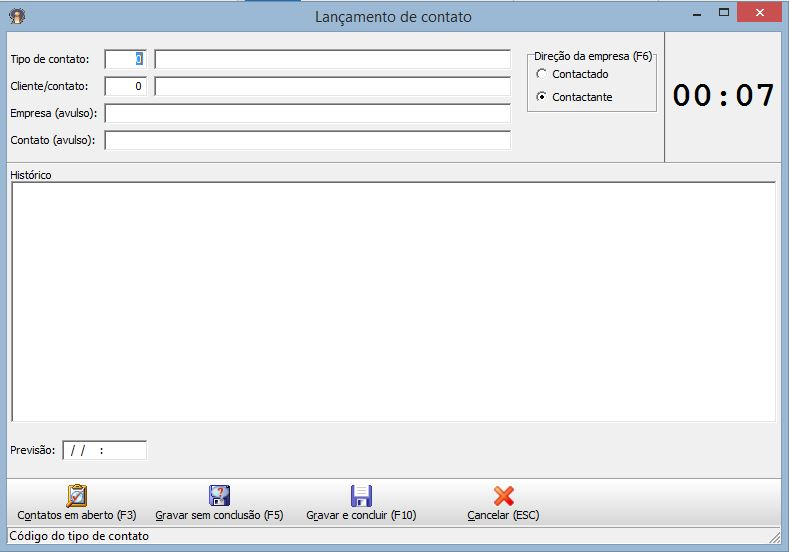
\includegraphics[scale=0.6]{figuras/jan_contatos_lancamento.jpg}
\caption{Janela de lançamento dos atendimentos}
\label{Fig:jan:contatos:lanca}
\end{figure}

\begin{figure}[!h]
\centering
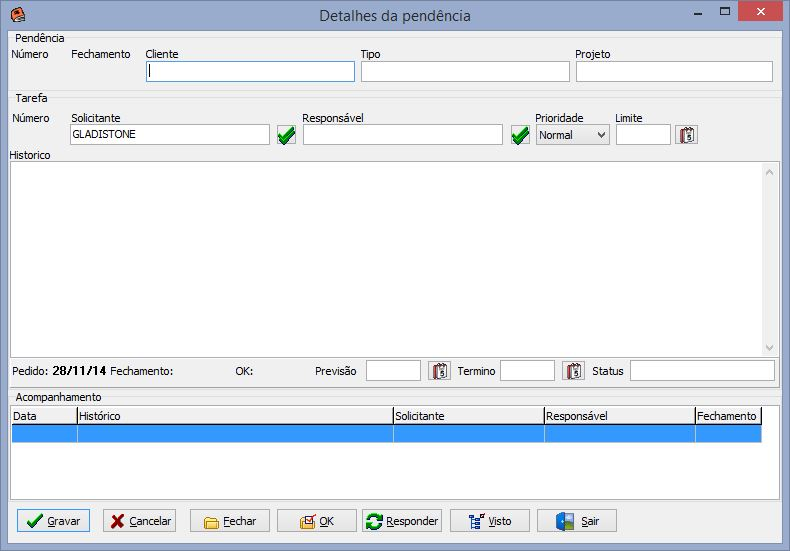
\includegraphics[scale=0.6]{figuras/jan_pendencias_lancamento.jpg}
\caption{Janela de lançamento das pendencias}
\label{Fig:jan:pendencias:lanca}
\end{figure}

Os atendimentos podem ser realizados através do telefone, acesso remoto via internet, e-mail ou presencial. Como pode ser observado na Figura \ref{Fig:atend11}, somente 3 tipos foram registrados no mês de novembro de 2014, mostrando que as comunicacões via e-mail não são registradas.

\begin{figure}[!h]
\centering
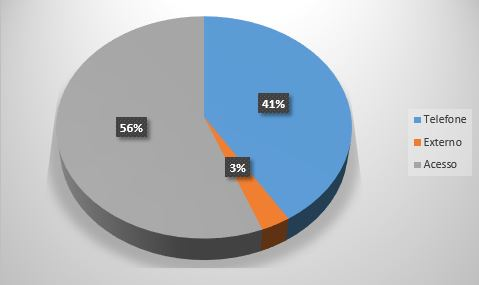
\includegraphics[scale=0.5]{figuras/atendimentos_por_tipo.jpg}
\caption{Atendimentos por tipo em novembro/2014}
\label{Fig:atend11}
\end{figure}

Outros problemas foram diagnosticados e estão relacionados na Tabela \ref{Tab:probl:atend}, sendo a falta de acompanhamento do andamento das solicitações e retorno ao cliente as mais críticas.

\begin{table}[h!]\footnotesize
\centering
\begin{tabular}
{
 	|p{14cm}|
}

	\hline
	\textbf{Problema diagnosticado}\\
	\hline

	Falta de registro de atendimento (para qualquer tipo)\\
	\hline

	Postergação de registro de atendimento (para qualquer tipo), que pode levar ao esquecimento (falta de registro)\\
	\hline
	
	Dados insuficientes sobre o contato\\
	\hline
	
	 Falta de acompanhamento do andamento das solicitações (fechamento dos registros de atendimento)\\
	\hline

	 Falta de retorno da situação das solicitações ao cliente\\
	\hline

	Tarefas originadas dos atendimentos, para o próprio departamento de suporte ou para outros departamentos, são registradas em um \sw separado e não há nenhuma rastreabilidade\\
	\hline

\end{tabular}
\caption {Problemas diagnosticados no departamento de suporte}
\label{Tab:probl:atend}
\end{table}

As seguintes ações devem ser tomadas para contonar os problemas diagnosticados:

\begin{itemize}

\item Todos os chamados técnicos deverão ser registrados no ato de sua execução (ligação, acesso remoto ou recebimento do e-mail), com exceção do atendimento externo que deve ser registrado no ato do retorno do técnico;

\item O máximo de informações possíveis precisa ser registrado no histórico do chamado;

\item A fusão entre o Contatos e o Pendências é extremamente necessária, a fim de criar um registro de todas as ações vinculadas naquele chamado, tornando-se obrigatório o registro de todas as ações realizadas por cada técnico que atender o chamado;

\item Qualquer nova informação de um chamado deve ser adicionada ao registro já aberto, sem a necessidade de abrir um novo chamado e permitindo a rastreabilidade;

\item Um departamento de Serviço de Atendimento ao Cliente (SAC) deverá ser criado e pelo menos uma pessoa deve ser colocada como responsável pelas suas atribuições;

\item O SAC realizará o fechamento do chamado junto ao cliente, consultando se realmente o problema foi solucionado e realizando pesquisas de satisfação e gerando indicadores de desempenho e qualidade (tempo médio de conclusão dos chamados, problemas mais ocorridos, cliente mais ativo, técnico mais ativo, etc);

\item Os clientes deverão receber um Documento de Abertura e Acompanhamento de Chamados, juntamente com o manual  do \sw, para que saibam exatamente como proceder para abrir e acompanhar um chamado;

\item Para uma melhor performance da equipe de suporte, deverá ser feito a gestão do conhecimento, documentando a resolução de cada problema que surja no atendimento do suporte técnico;

\item É necessária a elaboração de um fluxograma do atendimento, com as informações chaves de requisitos para abertura de chamados;

\item É necessária a elaboração de um fluxograma do atendimento de serviços diferenciados, tais como treinamentos, suportes avulsos, entrada de equipamento para concerto ou manutenção, entre outros, lembrando de acrescentar no fluxo a emissão da Ordem de Serviço;

\item Deverá ser realizado o acompanhamento dos clientes que não abrem chamado com o suporte há mais de 3 meses.

\end{itemize}

\subsection{Desenvolvimento}
\label{Sec:desenvolvimento}

Este departamento não tem contato direto com os clientes, pois todas as solicitações passam pelo departamento de suporte técnico. Porém, todas as solcitações de mudança ou correção de problemas nos \sws são resolvidas por este departamento e alguns atendimentos são repassados para o setor de desenvolvimento para resolução conjunta quando os técnicos não possuem conhecimento ou capacidade para tratá-los por si mesmos. 

As tarefas deste departamento são registradas no \sw Pendências mas, como já relatado anteriormente, não possuem relacionamento com os chamados abertos no \sw Contatos. Todos os problemas diagnosticados estão relacionados na Tabela \ref{Tab:probl:desenv}.

\begin{table}[h!]\footnotesize
\centering
\begin{tabular}
{
 	|p{14cm}|
}

	\hline
	\textbf{Problema diagnosticado}\\
	\hline

	Falta de posicionamento quanto ao andamento das solicitações\\
	\hline

	Falta de previsão de entrega das soluções\\
	\hline

	Falta de rastreabilidade entre abertura de chamados e tarefas\\
	\hline

\end{tabular}
\caption {Problemas diagnosticados no departamento de desenvolvimento}
\label{Tab:probl:desenv}
\end{table}

Para solucionar os problemas diagnosticados para este setor, além das ações ja citadas em \ref{Sec:suporte}, serão necessárias as seguintes ações:

\begin{itemize}

\item Criar processos para determinar a previsão de lançamento de versões de \sws;

\item Criar processos para determinar em qual versão determinada solicitação será incluída;

\item Integrar aos \sws de atendimento as informações de lançamento de versões e, consequentemente, a previsão das solicitacões.

\end{itemize}

\subsection{Financeiro}

O departamento financeiro lida com o cliente com uma frequência menor que os departamentos de suporte e desenvolvimento. Porém, os assuntos relacionados a este departamento podem gerar transtornos e prejuízos quando feitos de forma incorreta. Além disso, este departamento também é responsável por bloquear o atendimento aos clientes inadimplentes, portanto representa um papel importante nos processos descritos em \ref{Sec:suporte} e \ref{Sec:desenvolvimento}.

Nenhum atendimento ou tarefa relacionados a este departamento são registrados nos \sws de atendimento. Portanto, as ações necessárias para melhoria dos processos são:

\begin{itemize}

\item Registrar todo e qualquer contato com clientes nos \sws de atendimento;

\item Integrar as informações financeiras com os \sws de atendimento para que a liberação ou bloqueio seja feito automaticamente no ato da identificação do cliente.

\end{itemize}

\subsection{Marketing}

O departamento de marketing é o responsável, geralmente, pelo primeiro contato com o cliente. Durante as negociações de venda de \sw, é comum haver solicitações de modificações ou acertos sobre configurações, conversões de dados e treinamentos. Porém, nenhuma dessas informações são registradas nos \sws de atendimento. O mesmo ocorre na venda de equipamentos e outros serviços.

Portanto, as ações necessárias para melhoria dos processos são:

\begin{itemize}

\item Registrar os primeiros contatos com todos os prospectos, mesmo que não se tornem clientes;

\item Registrar toda e qualquer interação com os clientes, novos ou antigos;

\item Incluir nos registros as informações sobre negociação, possíveis modificações, conversões e outras condições estabelecidas durante ou após a venda.

\end{itemize}

\section{Análise SWOT}

A fim de resumir e melhor entender a análise organizacional e de processos realizada em \ref{Sec:analise:org}, foi desenvolvida a Tabela \ref{Tab:SWOT} com a análise SWOT.

\begin{table}[h!]\footnotesize
\centering
\begin{tabular}
{
	| >{\centering\arraybackslash}p{7cm}
	| >{\centering\arraybackslash}p{7cm}|
}
\hline

	Forças&
	Fraquezas\\
	\hline

	%Forças
	\begin{tabular}{p{6,8cm}}
	Comprometimento dos profissionais;\\
	Bom clima organizacional;\\
	Cultura de prezar pela excelência;\\
	Ser reconhecida através da sua confiabilidade e qualidade nos serviços.\\
	\end{tabular}&

	%Fraquezas
	\begin{tabular}{p{6,8cm}}
	Falta de informações no acompanhamento de solicitações;\\
	Ineficiência na comunicação com o cliente.\\
	\end{tabular}\\
	\hline

	Oportunidades&
	Ameaças\\
	\hline

	% Oportunidades
	\begin{tabular}{p{6,8cm}}
	Taxa de crescimento elevada nos últimos meses;\\
	Aumento no faturamento;\\
	Alta divulgação da marca, dentro e fora da sua própria cidade.\\
	\end{tabular}&

	% Ameaças
	\begin{tabular}{p{6,8cm}}
	Perder a confiabilidade dos clientes;\\
	Manchar a reputação;\\
	Sofrer queda nas vendas pela perda de indicações de clientes e parceiros insatisfeitos;\\
	Sofrer perda de clientes já estabelecidos por não prestar um bom atendimento.\\
	\end{tabular}\\
	\hline

\end{tabular}
\caption {Análise SWOT dos processos}
\label{Tab:SWOT}
\end{table}

%\bibliographystyle{plain}
%\bibliographystyle{bibstyle/latex8}     
%\bibliographystyle{apalike-url}     


\bibliographystyle{Bibliografia/apalike-pt}     

%\bibliographystyle{lastchecked}     
            
\bibliography{Bibliografia/research}

\end{document}